\documentclass[a4paper]{article}
\usepackage[utf8]{inputenc}
\usepackage[T1]{fontenc}
\usepackage[cache=false]{minted}
\usepackage[dvipsnames]{xcolor}
\usepackage{a4wide,syntax,listings,appendix,tikz,wrapfig,graphicx,hyperref}
\usepackage[margin=0.8in]{geometry}
\usepackage{pgfplots}
\usepackage{appendix}
\usepackage{diagbox}
\hypersetup{pdftitle={g08report},
pdfauthor={Pedro Mendes},
colorlinks=true,
urlcolor=blue,
linkcolor=black}
\usepackage{tikz}
\usetikzlibrary{matrix, calc, positioning}
\usepackage{fullpage,amsmath}
%\usetikzlibrary{arrows,positioning,automata,decorations.markings,shadows,shapes,calc}

\begin{document}

\title{Recomender System}
\author{Pedro Mendes (97144), Filipe Lucas (78775), Ricardo Pereira (86506)}
\date{\today}
\maketitle


\section{Serial}
There was no change in the serial version, as it is working as intended. One
important thing to note is that the MPI version uses the serial version when the
number of lines or columns in matrix A is less than the number of processors, as
it wouldn't make sense to use MPI for these cases.

\section{Decomposition}\label{s:decomposition}
When discussing how to perform the decomposition, the first implementation was
to transpose L so that it would be indexable as (k, i), which then aligned with
accessing R as (k, j). This had the advantage that matrices L and R could be
split among nodes and the calculations of $L$\textsuperscript{(t+1)} and
$R$\textsuperscript{(t+1)} could be made 100\% independently.  But this came
with a huge disadvantage: Matrix B could not be computed in parallel, all nodes
had to send their calculations of their slices of L and R to node 0 and this one
then computed matrix B alone and sent it back. This had so much overhead that
the sequential version could many times be faster.  Instead of trying to make it
work we decided to rewrite the program and split matrix $A$.

Matrix $A$ was then split in a checker board fashion, each node getting a zone
of A and the corresponding slices of L and R. The design was oriented to
facilitate the calculations of matrix B. This means that for some range of lines
of a, $[i, i'[$, and a range of columns, $[j, j'[$, assigned to node X, this
node will also have lines of $L$ from $i$ to $i'$ and all it's columns, and
columns of $R$ from $j$ to $j'$ and all of it's lines.

\begin{center}
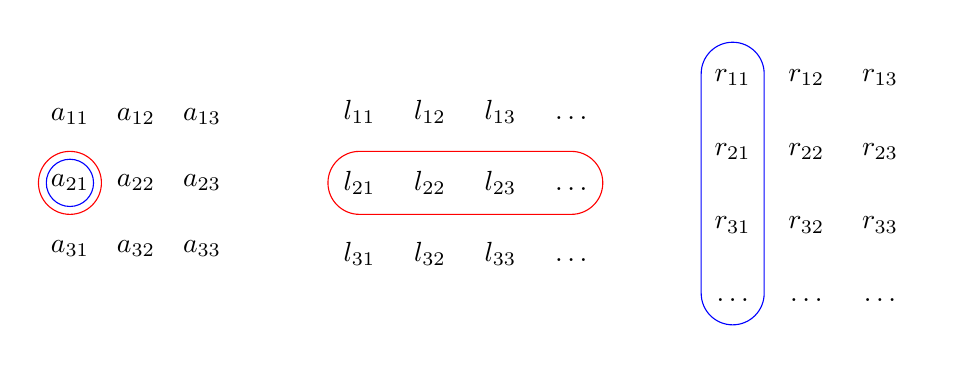
\begin{tikzpicture}[baseline=(A.center)]
 \tikzset{connect/.style={rounded corners=#1,
        to path=
        ($(\tikztostart)!-#1!(\tikztotarget)!-#1!-90:(\tikztotarget)$) --
        ($(\tikztotarget)!-#1!(\tikztostart)!-#1!90:(\tikztostart)$) --
        ($(\tikztotarget)!-#1!(\tikztostart)!#1!90:(\tikztostart)$) --
        ($(\tikztostart)!-#1!(\tikztotarget)!-#1!90:(\tikztotarget)$) --
        cycle (\tikztotarget)
 }}
 \tikzset{connect/.default=4mm}
 \tikzset{node style ge/.style={circle}}
 \matrix (A) [matrix of math nodes, nodes = {node style ge},,column sep=0 mm]
 {%
   a_{11} & a_{12} & a_{13}  \\
   a_{21} & a_{22} & a_{23}  \\
   a_{31} & a_{32} & a_{33}  \\
 };
 \draw[red] (A-2-1) circle (4mm) ;
 \draw[blue] (A-2-1) circle (3mm) ;

 \matrix (L) [right = of A-2-3.east, text depth= 1mm, text height = 3mm,
    matrix of math nodes, nodes = {node style ge},,column sep=0 mm]
 {%
    l_{11} & l_{12} & l_{13} & \ldots \\
    l_{21} & l_{22} & l_{23} & \ldots \\
    l_{31} & l_{32} & l_{33} & \ldots \\
 };
    \draw [red] (L-2-1) to[connect=4mm] (L-2-4) ;

 \matrix (R) [right = of L-2-4.east, text depth= 1mm, text height = 3mm,
    matrix of math nodes, nodes={node style ge},column sep=0 mm]
 {%
    r_{11} & r_{12} & r_{13}  \\
    r_{21} & r_{22} & r_{23}  \\
    r_{31} & r_{32} & r_{33}  \\
    \ldots & \ldots & \ldots  \\
 };
    \draw [blue] (R-1-1) to[connect=4mm] (R-4-1) ;
\end{tikzpicture}
\end{center}

With this decomposition the calculations of matrix $B$ can be done independently
by the nodes, on the other hand this means that communication had to be shifted
somewhere else, this place being in the calculations of L\textsuperscript{(t+1)}
and R\textsuperscript{(t+1)}. The way it works is since these nodes don't have
enough of matrix $A$ to calculate their parts of L or R, they do as much as
possible and in the end we make use of \texttt{MPI\_Allreduce} to sum all their
values.

\subsection{MPI Reduction}
Taking advantage of the checker board layout each node only has to reduce with
nodes that share their slice of L/R.

\begin{center}
\begin{tikzpicture}[baseline=(A.center)]
 \tikzset{connect/.style={rounded corners=#1,
        to path=
        ($(\tikztostart)!-#1!(\tikztotarget)!-#1!-90:(\tikztotarget)$) --
        ($(\tikztotarget)!-#1!(\tikztostart)!-#1!90:(\tikztostart)$) --
        ($(\tikztotarget)!-#1!(\tikztostart)!#1!90:(\tikztostart)$) --
        ($(\tikztostart)!-#1!(\tikztotarget)!-#1!90:(\tikztotarget)$) --
        cycle (\tikztotarget)
 }}
 \tikzset{connect/.default=4mm}
 \tikzset{node style ge/.style={circle}}
 \matrix (L) [text depth= 1mm, text height = 3mm,
    matrix of math nodes, nodes = {node style ge},,column sep=0 mm]
 {%
    l_{11} & l_{12} & l_{13} & \ldots \\
    l_{21} & l_{22} & l_{23} & \ldots \\
    l_{31} & l_{32} & l_{33} & \ldots \\
 };
 \draw [thick,red] (L-1-1) to[connect=4mm] (L-1-4) ;
 \draw [thick,blue] (L-2-1) to[connect=4mm] (L-2-4) ;
 \draw [thick,green] (L-3-1) to[connect=4mm] (L-3-4) ;

 \matrix (R) [right = of L-2-4.east, text depth= 1mm, text height = 3mm,
    matrix of math nodes, nodes={node style ge},column sep=0 mm]
 {%
    r_{11} & r_{12} & r_{13}  \\
    r_{21} & r_{22} & r_{23}  \\
    r_{31} & r_{32} & r_{33}  \\
    \ldots & \ldots & \ldots  \\
 };
    \draw [thick,orange] (R-1-1) to[connect=4mm] (R-4-1) ;
    \draw [thick,violet] (R-1-2) to[connect=4mm] (R-4-2) ;
    \draw [thick,yellow] (R-1-3) to[connect=4mm] (R-4-3) ;
\end{tikzpicture}
\end{center}

If we give each line and row of $L$ and $R$ a colour, we can than define a node
as a combination of 2 colours, and then it only has to communicate with nodes
that share a colour with it. For example, given the following table

\begin{center}
    \begin{tabular}{|c|c|c|c|}
        \hline
        \diagbox{R}{L} & red & blue & green \\\hline
        orange         & 0   & 1    & 2     \\\hline
        violet         & 3   & 4    & 5     \\\hline
        yellow         & 6   & 7    & 8     \\\hline
    \end{tabular}
\end{center}

We can see that node 0 only needs to communicate with nodes 1 and 2 to calculate
matrix L and nodes 3 and 6 to calculate matrix R.

\subsection{Memory}

Another huge advantage of this decomposition is that at no point (excluding the
very end of the algorithm) does any node have in memory an entire matrix.

In total the amount of spent memory is relative to the amount of processes, each
process will at most have $\sqrt{\#processors}$ lines of matrix L and
$\sqrt{\#processors}$ rows of matrix R. Of matrix \texttt{A} and \texttt{B} only the
the areas defined previously (Section~\ref{s:decomposition}) will be stored.

At the end of the computation, all matrices except B are freed and node 0
gathers the parts of matrix B the other nodes calculated, so it can finally print
the output.

\section{Load Balancing}
In the cases that the lines and columns are not dividable by the number of nodes
the the first X nodes take one more line/column where X is the remainder of the
division. This has the convenient property of helping during parsing, since node
0 has always the largest area of matrix A it can always accumulate the values
that belong to other nodes without having to overcommit memory.

\section{Performance}
Benchmarks were made for the three biggest instances:
\texttt{inst1000-80000-20-10-1000}, \texttt{inst20000-10000-40-2-50} and,
\texttt{inst60000-2000-200-10-20}. Since the program can only make use of
numbers of processors whose square root is an integer, the performance gains
from using 32 nodes over using 16 are not great, on the other hand when bumping
the number to 64 nodes, since 64 has an integer root, the performance gains are
much better.  The times for these benchmarks can be seen in
Appendix~\ref{app:bench1}.

To show a more realistic performance graph we also benchmarked with the number
of nodes with integer square roots. These can be seen in
Appendix~\ref{app:bench1}. One interesting note is that the performance of 36
and 49 is worse then the performance of 16. We suspect this might be because the
machines used have 4 cores each, so powers of 2 create more even distributions,
improving comunication performance.

\section{Future Work}
There are 2 major flaws in the implementation that, given enough time, could be fixed.

The first is that the number of allowed nodes is very strict. Only numbers whose square
root is an integer can be used, excess nodes are discarded.

The other improvement that could be made is node 0 not aggregating the elements of B from
the other nodes as this might be too much for some instances.

\begin{appendices}
\section{Benchmarks: Powers of two}\label{app:bench1}

\begin{figure}[H]
    \centering

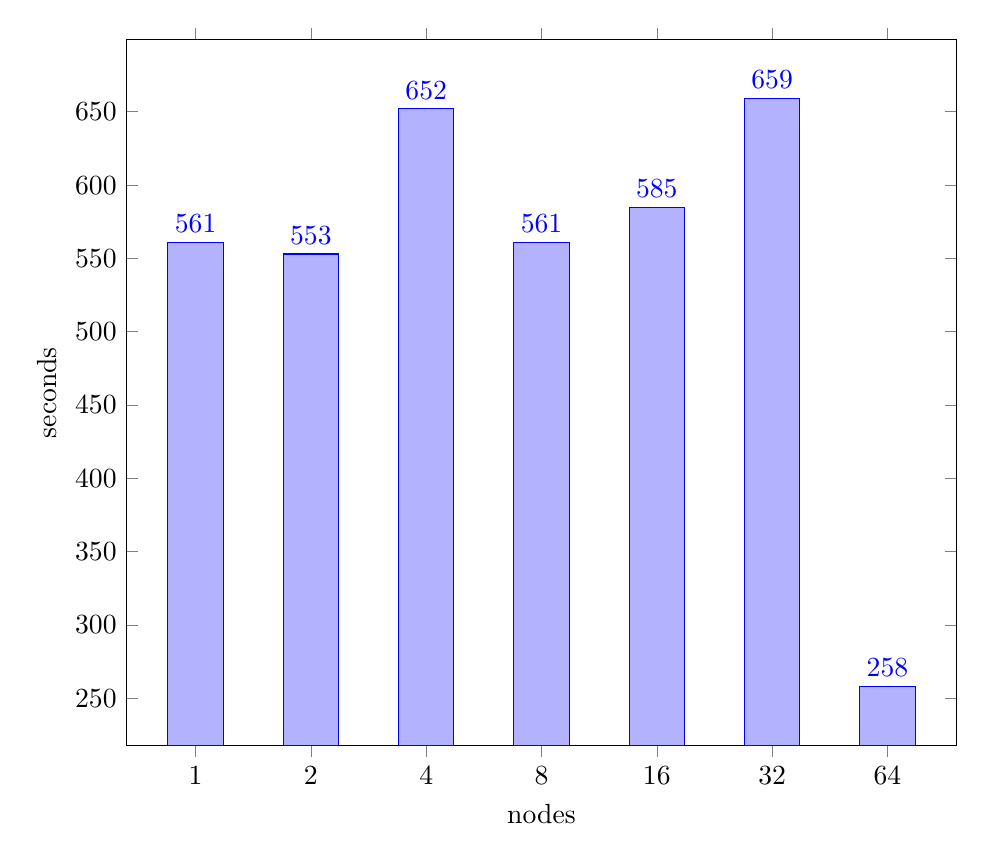
\begin{tikzpicture}
    \begin{axis}[
            ybar,
            enlargelimits=true,
            bar width=20pt,
            width=\textwidth,
            height=300pt,
            legend style={at={(0.5,-0.15)}, anchor=north,legend columns=-1},
            ylabel={seconds},
            xlabel={nodes},
            symbolic x coords={1,2,4,8,16,32,64},
            xtick=data,
            nodes near coords,
            nodes near coords align={vertical},
        ]
\addplot coordinates {
(1,561)	% ./guided_new_parser_bin
(2,553)	% ./guided_new_parser_bin
(4,652)	% ./guided_new_parser_bin
(8,561)	% ./guided_new_parser_bin
(16,585)	% ./guided_new_parser_bin
(32,659)	% ./guided_new_parser_bin
(64,258)	% ./guided_new_parser_bin
};
    \end{axis}
\end{tikzpicture}    
\caption{inst1000-80000-20-10-1000}
\label{fig:1000}
\end{figure}
\begin{figure}[H]
    \centering
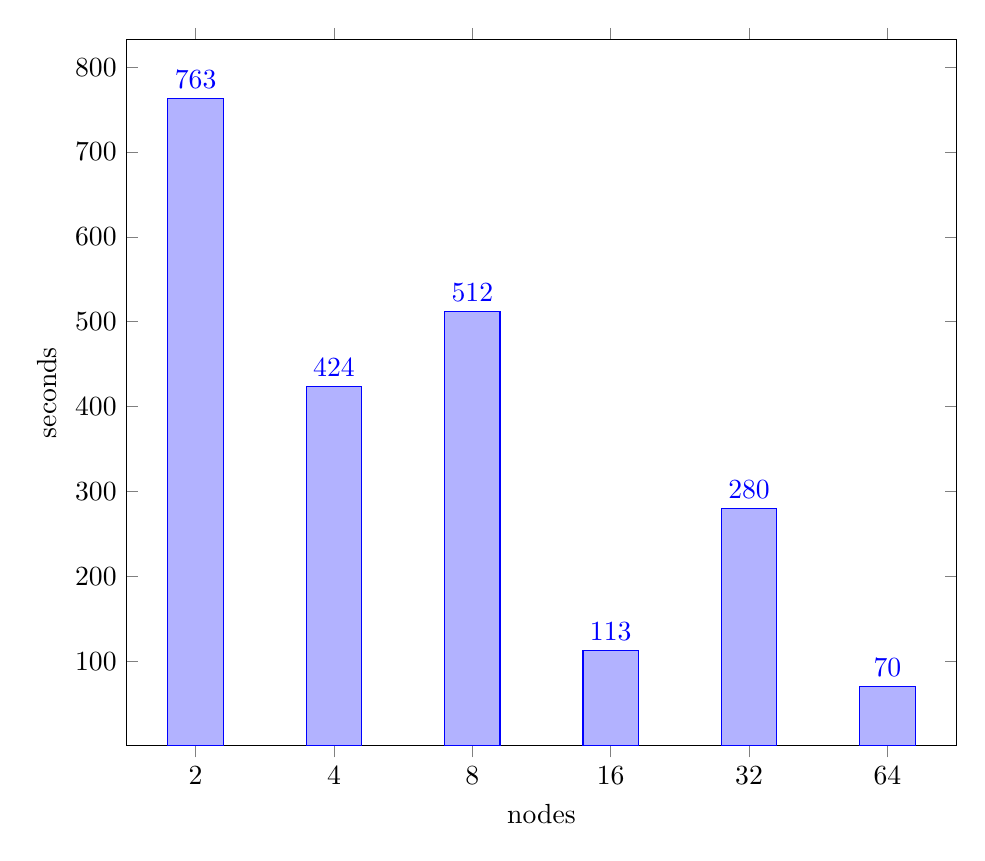
\begin{tikzpicture}
    \begin{axis}[
            ybar,
            enlargelimits=true,
            bar width=20pt,
            width=\textwidth,
            height=300pt,
            legend style={at={(0.5,-0.15)}, anchor=north,legend columns=-1},
            ylabel={seconds},
            xlabel={nodes},
            symbolic x coords={2,4,8,16,32,64},
            xtick=data,
            nodes near coords,
            nodes near coords align={vertical},
        ]
\addplot coordinates {
(2,763)	% ./guided_new_parser_bin
(4,424)	% ./guided_new_parser_bin
(8,512)	% ./guided_new_parser_bin
(16,113)	% ./guided_new_parser_bin
(32,280)	% ./guided_new_parser_bin
(64,70)	% ./guided_new_parser_bin
};
    \end{axis}
\end{tikzpicture}
    \caption{inst20000-10000-40-2-50}
    \label{fig:20000}
\end{figure}
\input{benchmarks/bench-60000}

\section{Benchmarks: Integer Square Roots}\label{app:bench1}

\begin{figure}[H]
    \centering

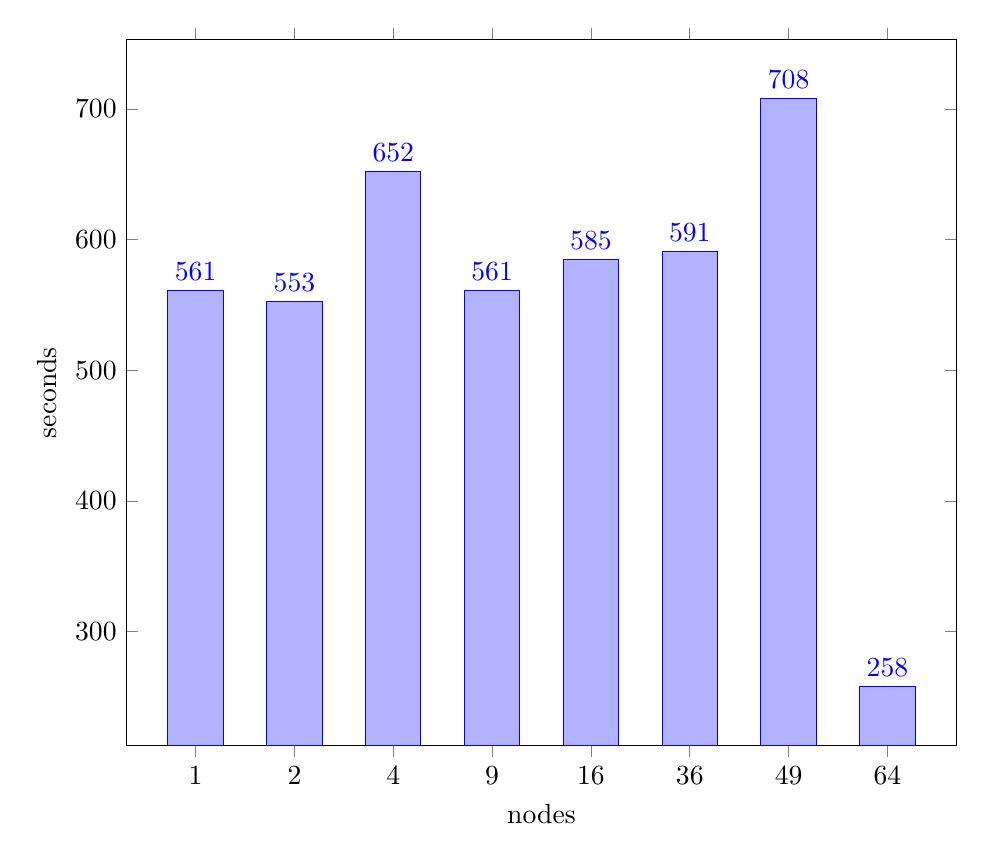
\begin{tikzpicture}
    \begin{axis}[
            ybar,
            enlargelimits=true,
            bar width=20pt,
            width=\textwidth,
            height=300pt,
            legend style={at={(0.5,-0.15)}, anchor=north,legend columns=-1},
            ylabel={seconds},
            xlabel={nodes},
            symbolic x coords={1,2,4,9,16,36,49,64},
            xtick=data,
            nodes near coords,
            nodes near coords align={vertical},
        ]
\addplot coordinates {
(1,561)	% ./guided_new_parser_bin
(2,553)	% ./guided_new_parser_bin
(4,652)	% ./guided_new_parser_bin
(9,561)	% ./guided_new_parser_bin
(16,585)	% ./guided_new_parser_bin
(36,591)	% ./guided_new_parser_bin
(49,708)
(64,258)	% ./guided_new_parser_bin
};
    \end{axis}
\end{tikzpicture}    
\caption{inst1000-80000-20-10-1000}
\label{fig:1000}
\end{figure}
\begin{figure}[H]
    \centering
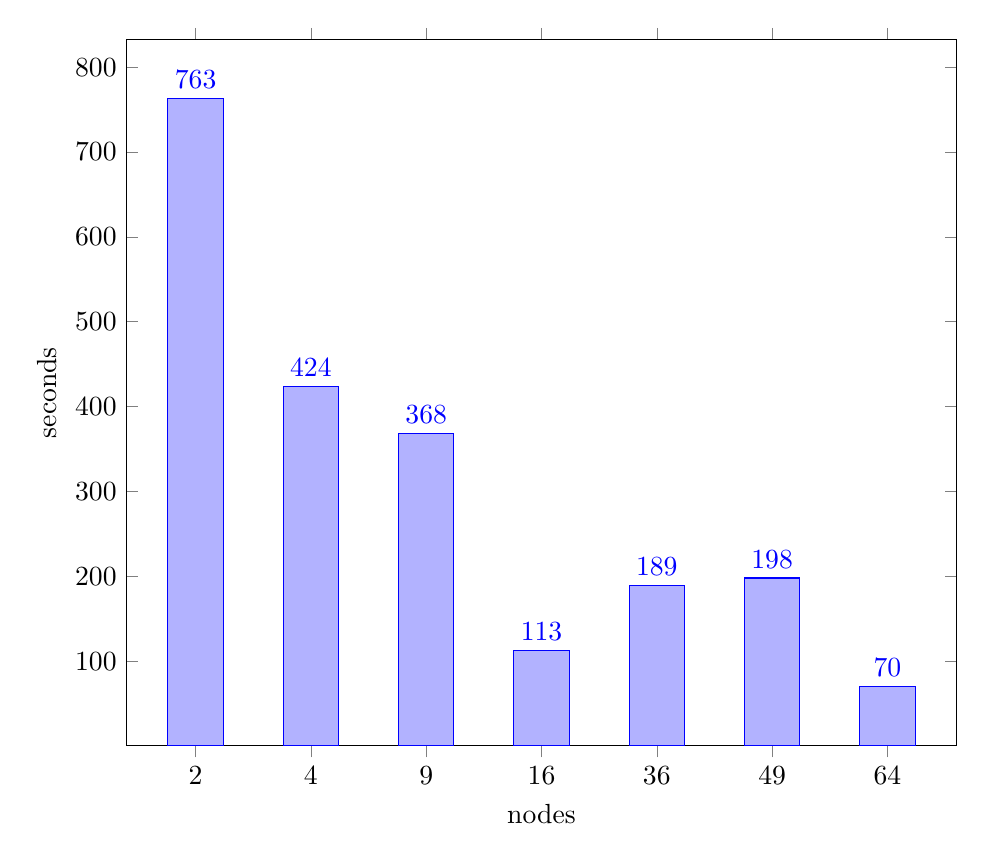
\begin{tikzpicture}
    \begin{axis}[
            ybar,
            enlargelimits=true,
            bar width=20pt,
            width=\textwidth,
            height=300pt,
            legend style={at={(0.5,-0.15)}, anchor=north,legend columns=-1},
            ylabel={seconds},
            xlabel={nodes},
            symbolic x coords={2,4,9,16,36,49,64},
            xtick=data,
            nodes near coords,
            nodes near coords align={vertical},
        ]
\addplot coordinates {
(2,763)	% ./guided_new_parser_bin
(4,424)	% ./guided_new_parser_bin
(9,368)	% ./guided_new_parser_bin
(16,113)	% ./guided_new_parser_bin
(36,189)	% ./guided_new_parser_bin
(49,198)
(64,70)	% ./guided_new_parser_bin
};
    \end{axis}
\end{tikzpicture}
    \caption{inst20000-10000-40-2-50}
    \label{fig:20000}
\end{figure}
\begin{figure}[H]
    \centering
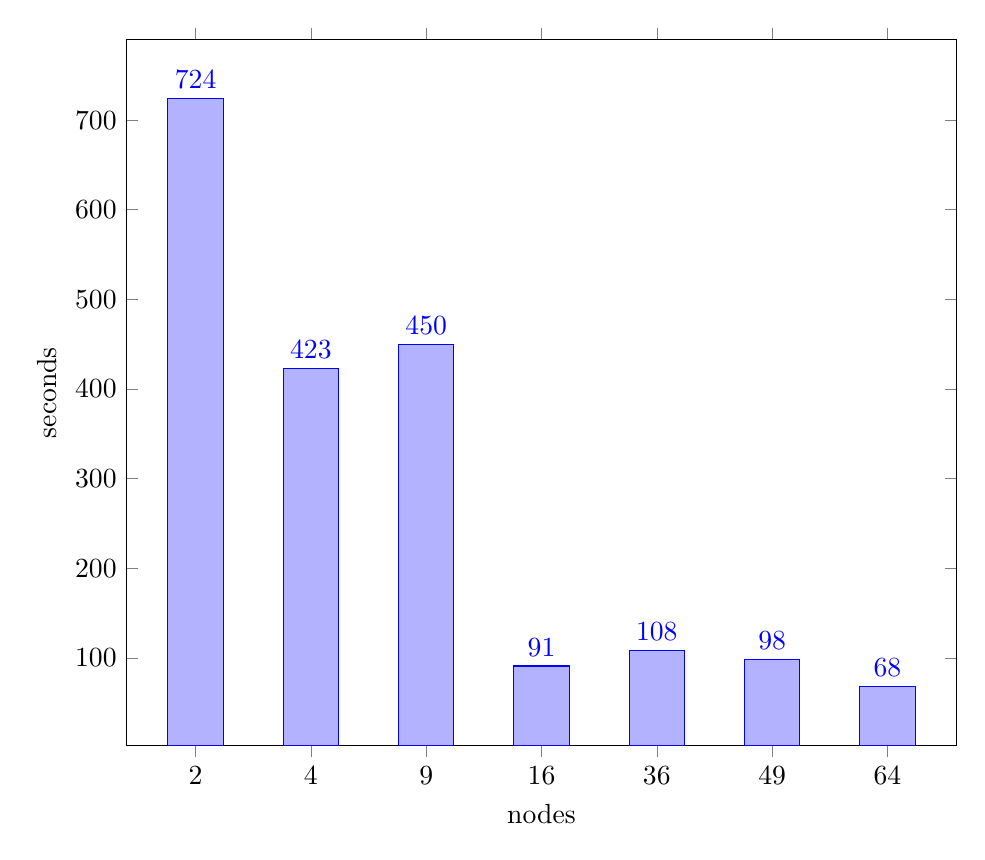
\begin{tikzpicture}
    \begin{axis}[
            ybar,
            enlargelimits=true,
            bar width=20pt,
            width=\textwidth,
            height=300pt,
            legend style={at={(0.5,-0.15)}, anchor=north,legend columns=-1},
            ylabel={seconds},
            xlabel={nodes},
            symbolic x coords={2,4,9,16,36,49,64},
            xtick=data,
            nodes near coords,
            nodes near coords align={vertical},
        ]
\addplot coordinates {
(2,724)	% ./guided_new_parser_bin
(4,423)	% ./guided_new_parser_bin
(9,450)	% ./guided_new_parser_bin
(16,91)	% ./guided_new_parser_bin
(36,108)	% ./guided_new_parser_bin
(49,98)
(64,68)	% ./guided_new_parser_bin
};
    \end{axis}
\end{tikzpicture}
    \caption{inst60000-2000-200-10-20}
    \label{fig:60000}
\end{figure}

\end{appendices}
\newpage

\end{document}
